\documentclass[journal]{IEEEtran}
\usepackage{amsmath,amssymb}
\usepackage{amsthm}
\usepackage{url}
\usepackage{graphicx}
\usepackage{booktabs}
\usepackage{hyperref}

\begin{document}

\title{Extending the Oracle Approximating Shrinkage to General Distributions}
\author{Michael~J.~Lewis,~\IEEEmembership{Independent Researcher}%
\thanks{Manuscript received October 2026.}}

\maketitle

\begin{abstract}
The Oracle Approximating Shrinkage (OAS) estimator provides a closed-form, data-driven
shrinkage intensity for regularizing sample covariance matrices toward a scaled identity
target, but its derivation assumes Gaussian data.
In practice, financial returns, neural signals, and many other high-dimensional datasets
exhibit heavy tails and non-zero kurtosis, violating this assumption.
We extend OAS to any distribution with finite fourth moments by incorporating a correction
term $\alpha$ built from the fourth-order joint cumulants of the data.
The correction vanishes under Gaussianity, recovering the OAS formula as a special
case; it admits a consistent $O(np)$ sample estimator and satisfies $\rho\in[0,1]$ exactly
for both the population cumulant and its sample analogue.
Simulations and an equity-returns study confirm that the correction closes the gap between
OAS and the Ledoit--Wolf estimator under non-Gaussian data, with OAS-Extended
performing comparably across all tested settings.
The contribution is a principled correction for OAS practitioners facing heavy-tailed data;
structurally, it is distinct from prior work extending Ledoit--Wolf to elliptical
distributions, which optimizes against a fixed oracle target and yields a different
closed-form formula.
\end{abstract}

\begin{IEEEkeywords}
covariance matrix estimation, shrinkage estimation, Oracle Approximating Shrinkage,
fourth-order cumulants, non-Gaussian distributions, heavy tails, high-dimensional statistics,
portfolio optimization
\end{IEEEkeywords}

\section{Introduction}\label{sec-intro}

Estimating a covariance matrix from data is a fundamental task across a wide range of
disciplines, including portfolio optimization \cite{LW2004}, signal processing \cite{OAS},
and neuroscience.
In the classical low-dimensional regime, the sample covariance matrix $\hat{S}$ is a
consistent and unbiased estimator of the true covariance $\Sigma$.
However, in the modern high-dimensional setting where the number of variables $p$ is
comparable to or exceeds the number of observations $n$, $\hat{S}$ becomes poorly
conditioned or singular, and its eigenvalues are known to be severely dispersed relative
to those of $\Sigma$.

Shrinkage estimators address this by forming a convex combination
\begin{equation*}
\hat{\Sigma} = (1 - \rho)\hat{S} + \rho \hat{F},
\end{equation*}
where $\hat{F}$ is a well-conditioned target matrix and $\rho \in [0,1]$ is a shrinkage
intensity.
The celebrated Ledoit--Wolf (LW) estimator \cite{LW2004} chooses $\rho$ to minimize the
expected Frobenius loss $E[\lVert \hat{\Sigma} - \Sigma \rVert_F^2]$ against the oracle
target $\hat{F} = (\operatorname{Tr}(\Sigma)/p)\,I$.
The Oracle Approximating Shrinkage (OAS) estimator of Chen et al.\ \cite{OAS} takes a
different approach: it uses the data-dependent target
$\hat{F} = (\operatorname{Tr}(\hat{S})/p)\,I$ and derives $\rho$ via a fixed-point
iteration that converges to a closed-form expression.
This distinction --- random versus fixed target --- leads to structurally different
formulas and different finite-sample behavior, with OAS typically outperforming LW
at small $n/p$ ratios under Gaussian data.

Both estimators were originally derived under the assumption of multivariate Gaussian data.
In many practical settings this assumption fails.
Financial asset returns are well-documented to exhibit excess kurtosis and heavy tails.
More broadly, any distribution in the elliptical family --- including the multivariate
Student-$t$ --- introduces fourth-order cumulant structure that the Gaussian-derived
formulas ignore.
Under such distributions, applying the OAS formula amounts to a misspecified estimator,
and the resulting shrinkage intensity is suboptimal.

The key insight is that the Gaussian derivation of OAS depends on two expectations ---
$E[\operatorname{Tr}(\hat{S}^2)]$ and $E[\operatorname{Tr}^2(\hat{S})]$ --- each of which
acquires an additional term $\alpha/n$ under a general distribution, where
$\alpha = \sum_{i,j} \kappa(X_i, X_i, X_j, X_j)$ aggregates the fourth-order joint
cumulants of the data.
Incorporating this term propagates through the fixed-point iteration and yields a
corrected closed-form shrinkage intensity that reduces to the OAS formula when
$\alpha = 0$.
We also provide a consistent sample estimator $\hat{\alpha}$ and prove that the corrected
formula preserves $\rho \in [0,1]$ for both the population cumulant and the sample
estimator, so an OAS practitioner facing non-Gaussian data can adopt the extended
formula without changing frameworks.

\section{Related Work}\label{sec-related}

The closest prior work is the extension of LW shrinkage to elliptical distributions by
Ollila and collaborators \cite{Ollila2017,OllilaRaninen2019,Ollila2023}, which minimizes
\begin{equation*}
E\!\left[\lVert (1-\rho)\hat{S} + \rho\mu I - \Sigma \rVert_F^2\right]
\end{equation*}
where $\mu = \operatorname{Tr}(\Sigma)/p$ is a \emph{fixed} oracle scalar, yielding a
closed-form expression parameterized by the scalar elliptical kurtosis $\kappa$ and
the sphericity $\gamma = p\operatorname{Tr}(\Sigma^2)/\operatorname{Tr}^2(\Sigma)$.

The OAS framework of \cite{OAS} differs structurally: the target
$\hat{F} = (\operatorname{Tr}(\hat{S})/p)\,I$ is \emph{random and data-dependent} rather
than the oracle $\mu I$.
This changes the optimization problem and produces a different formula via fixed-point
iteration; the two approaches are not equivalent even in the Gaussian case.
Consequently, the elliptical results of \cite{Ollila2017,OllilaRaninen2019} do not imply
an extension of OAS, and to the best of our knowledge the present work is the first to
provide one.

Our result is also more general in distributional scope.
The Ollila line restricts to elliptical distributions, for which
$\kappa(X_i,X_i,X_j,X_j) = \kappa(\Sigma_{ii}\Sigma_{jj}+2\Sigma_{ij}^2)$
for a scalar $\kappa$.
Our result holds for any distribution with finite fourth moments, where $\alpha$ need not
have this constrained form; elliptical distributions are a special case.

\section{Corrected Oracle Intensity}\label{sec-formulation}

\paragraph{Setup and notation.}
Let $X^1,\ldots,X^n\in\mathbb{R}^p$ be i.i.d.\ draws from a centered distribution with
covariance $\Sigma$ and finite fourth moments.
The sample covariance is
\begin{equation*}
\hat{S} = \frac{1}{n}\sum_{k=1}^n X^k(X^k)^T,
\end{equation*}
and the shrinkage target is $\hat{F}=\frac{\operatorname{Tr}(\hat{S})}{p}I$.
The setup and following equations follow \cite{OAS}:
\begin{align}
\rho_O &= \frac{E[\operatorname{Tr}((\Sigma-\hat{S})(\hat{F}-\hat{S}))]}{E[\lVert\hat{S}-\hat{F}\rVert_F^2]}, \label{eq:oracle}\\
E[\lVert\hat{S}-\hat{F}\rVert_F^2] &= E[\operatorname{Tr}(\hat{S}^2)] - \frac{E[\operatorname{Tr}^2(\hat{S})]}{p}. \label{eq:denom}
\end{align}
Here we depart from \cite{OAS}: rather than assuming Gaussianity, we allow the
distribution to be arbitrary with finite fourth moments.
Observe that
\begin{align}
E[\operatorname{Tr}(\hat{S}^2)]
&= \sum_{i,j}\frac{1}{n^2}\sum_{k,l} E[X_i^k X_j^k X_i^l X_j^l] \nonumber\\
&= \frac{n-1}{n}\sum_{i,j}\Sigma_{ij}^2
   + \frac{1}{n}\sum_{i,j}E[X_i^2 X_j^2] \nonumber\\
&= \frac{n-1}{n}\operatorname{Tr}(\Sigma^2)
   + \frac{1}{n}\sum_{i,j}E[X_i^2 X_j^2]. \label{eq:trS2expand}
\end{align}
Similarly,
\begin{align}
E[\operatorname{Tr}^2(\hat{S})]
&= \sum_{i,j}\frac{1}{n^2}\sum_{k,l}E[(X_i^k)^2(X_j^l)^2] \nonumber\\
&= \frac{n-1}{n}\operatorname{Tr}^2(\Sigma)
   + \frac{1}{n}\sum_{i,j}E[X_i^2 X_j^2]. \label{eq:tr2Sexpand}
\end{align}
The term $\sum_{i,j}E[X_i^2 X_j^2]$ appears in both expansions.
For a centered distribution with finite fourth moments,
\begin{equation}
E[X_i^2 X_j^2] = \Sigma_{ii}\Sigma_{jj} + 2\Sigma_{ij}^2
  + \kappa(X_i,X_i,X_j,X_j), \label{eq:fourthmoment}
\end{equation}
where $\kappa(X_i,X_i,X_j,X_j)$ is the fourth-order joint cumulant, vanishing under
Gaussianity. Letting $\alpha=\sum_{i,j}\kappa(X_i,X_i,X_j,X_j)$,
\begin{equation}
\sum_{i,j}E[X_i^2 X_j^2]
  = \operatorname{Tr}^2(\Sigma)+2\operatorname{Tr}(\Sigma^2)+\alpha. \label{eq:sumfourth}
\end{equation}
Substituting \eqref{eq:sumfourth} into \eqref{eq:trS2expand} and \eqref{eq:tr2Sexpand},
\begin{align}
E[\operatorname{Tr}(\hat{S}^2)] &= \tfrac{n+1}{n}\operatorname{Tr}(\Sigma^2)
  +\tfrac{1}{n}\operatorname{Tr}^2(\Sigma)+\tfrac{\alpha}{n}, \label{eq:trS2}\\
E[\operatorname{Tr}^2(\hat{S})] &= \operatorname{Tr}^2(\Sigma)
  +\tfrac{2}{n}\operatorname{Tr}(\Sigma^2)+\tfrac{\alpha}{n}, \label{eq:tr2S}
\end{align}
matching the Gaussian results of \cite{OAS} up to the $\alpha/n$ term.
Substituting into \eqref{eq:oracle} and simplifying yields the corrected oracle intensity:
\begin{equation}
\label{opt_rho}
\rho_O = \frac{(1-\tfrac{2}{p})\operatorname{Tr}(\Sigma^2)+\operatorname{Tr}^2(\Sigma)+\alpha(1-\tfrac{1}{p})}{(n+1-\tfrac{2}{p})\operatorname{Tr}(\Sigma^2)+(1-\tfrac{n}{p})\operatorname{Tr}^2(\Sigma)+\alpha(1-\tfrac{1}{p})}.
\end{equation}

\section{OAS-Extended}\label{sec-extension}

We now apply the OAS fixed-point framework of \cite{OAS} to the corrected oracle formula
\eqref{opt_rho}.
As in \cite{OAS}, we have
\begin{align}
\hat{\rho}_{j+1} &= \frac{(1-\tfrac{2}{p})\operatorname{Tr}(\hat{\Sigma}_j\hat{S})
  +\operatorname{Tr}^2(\hat{\Sigma}_j)+\alpha(1-\tfrac{1}{p})}
  {(n+1-\tfrac{2}{p})\operatorname{Tr}(\hat{\Sigma}_j\hat{S})
  +(1-\tfrac{n}{p})\operatorname{Tr}^2(\hat{\Sigma}_j)+\alpha(1-\tfrac{1}{p})},
  \label{rho_eval}\\
\hat{\Sigma}_{j+1} &= (1-\hat{\rho}_{j+1})\hat{S}+\hat{\rho}_{j+1}\hat{F}, \label{sigma_eval}
\end{align}
which replaces $\operatorname{Tr}(\Sigma)$ and $\operatorname{Tr}(\Sigma^2)$ with
$\operatorname{Tr}(\hat{\Sigma}_j)$ and $\operatorname{Tr}(\hat{\Sigma}_j\hat{S})$.
Let
\begin{equation}
\hat{\phi} = \frac{\operatorname{Tr}(\hat{S}^2)-\operatorname{Tr}^2(\hat{S})/p}{M}, \quad
M = (1-\tfrac{2}{p})\operatorname{Tr}(\hat{S}^2)+\operatorname{Tr}^2(\hat{S}),
\end{equation}
and $\beta=\alpha(1-1/p)/M$.
Substituting \eqref{sigma_eval} into \eqref{rho_eval} and simplifying,
\begin{equation}
\hat{\rho}_{j+1} = \frac{1+\beta-(1-\tfrac{2}{p})\hat{\phi}\hat{\rho}_j}
  {1+\beta+n\hat{\phi}-(n+1-\tfrac{2}{p})\hat{\phi}\hat{\rho}_j}.
\end{equation}
The change of variables
\begin{equation}
b_j = \frac{1}{1+\beta-(n+1-\tfrac{2}{p})\hat{\phi}\hat{\rho}_j}
\end{equation}
reduces this to the linear recurrence
\begin{equation}
b_{j+1} = \frac{n\hat{\phi}}{1+\beta-(1-\tfrac{2}{p})\hat{\phi}}\,b_j
  + \frac{1}{1+\beta-(1-\tfrac{2}{p})\hat{\phi}}.
\end{equation}
Its limit gives
\begin{equation}
\label{new_OAS}
\rho_{\text{OAS-E}} = \min\!\left(1,\, \frac{1+\beta}{(n+1-\tfrac{2}{p})\,\hat{\phi}}\right),
\end{equation}
the OAS-Extended estimator, recovering standard OAS when $\beta=0$.

\paragraph{Sample estimator for $\alpha$.}
The natural moment estimator simplifies to
\begin{equation}
\hat{\alpha} = \widehat{\operatorname{Var}}(\lVert X\rVert^2) - 2\operatorname{Tr}(\hat{S}^2),
\end{equation}
where
$\widehat{\operatorname{Var}}(\lVert X\rVert^2)
  = \frac{1}{n}\sum_k\lVert X^k\rVert^4 - \operatorname{Tr}^2(\hat{S})$
is the sample variance of squared norms, convergent to $\alpha$ by the law of large numbers.
This has a natural interpretation: $\hat{\alpha}$ measures the excess squared-norm variance
beyond what a Gaussian with covariance $\hat{S}$ would produce
($2\operatorname{Tr}(\hat{S}^2)$ being the Gaussian value), and is computable in $O(np)$
additional time once $\hat{S}$ is formed.
Appendix~\ref{app:proof} shows that $1+\hat{\beta}\geq0$ holds exactly for every finite
sample, so $\rho_{\text{OAS-E}}\in[0,1]$ without clamping.

\section{Simulation Study}\label{sec-simulation}

We evaluate OAS-Extended against OAS \cite{OAS}, RBLW \cite{OAS}, LW \cite{LW2004},
and the sample covariance.
All experiments use $p=120$ with AR(1) covariance $\Sigma_{ij}=0.5^{|i-j|}$,
$n/p\in\{0.25,0.5,1,2,5\}$, and 500 independent trials per setting.
The smallest ratio $n/p=0.25$ corresponds to $n=30$ observations, ensuring the
sample is large enough for stable estimation of $\hat{\alpha}$ while remaining well
into the high-dimensional regime where $\hat{S}$ is singular.
Performance is measured by normalized Frobenius loss
$\lVert\hat{\Sigma}-\Sigma\rVert_F/\lVert\Sigma\rVert_F$.

Three distributions are tested: Gaussian ($\alpha=0$) as a sanity check; multivariate
Student-$t$ with $\nu=10$ degrees of freedom (excess kurtosis $=1$); and $\nu=5$
(excess kurtosis $=6$), both scaled so $\operatorname{Cov}(X)=\Sigma$ exactly.
For a multivariate Student-$t$ with $\nu$ degrees of freedom,
$\alpha = \frac{2}{\nu-4}[\operatorname{Tr}^2(\Sigma)+2\operatorname{Tr}(\Sigma^2)]$,
which grows rapidly as $\nu\to4$, explaining why the correction is substantially larger
under $t(\nu\!=\!5)$ than $t(\nu\!=\!10)$.

Table~\ref{tab:sim} reports mean losses.
Under Gaussian data all four shrinkage estimators perform comparably, confirming no bias
when $\alpha=0$.
Under non-Gaussian data four findings stand out.
First, OAS-Extended recovers the performance lost by OAS's Gaussian misspecification,
performing comparably to LW across all settings.
Second, both dominate OAS substantially under $t(\nu\!=\!5)$: losses fall by 46--48\%
at $n/p\leq0.5$, $\sim$36\% at $n/p=1$, $\sim$24\% at $n/p=2$, and $\sim$16\% at $n/p=5$.
Third, RBLW performs comparably to OAS under non-Gaussian data, confirming that
neither the Rao-Blackwell construction of RBLW nor the fixed-point iteration of OAS
provides a non-Gaussian correction.
Fourth, the improvement of OAS-Extended over OAS grows with kurtosis and shrinks
as $n/p$ increases, exactly as predicted by the theory.
Figure~\ref{fig:sim} shows loss curves and relative improvement over the full range
$n/p\in[0.25,10]$.

\begin{table}[ht]
\centering
\caption{Mean normalized Frobenius loss ($p=120$, 500 trials). Lower is better.}
\label{tab:sim}
\begin{tabular}{clccccc}
\toprule
$n/p$ & Distribution & S & LW & RBLW & OAS & OAS-E \\
\midrule
0.25 & Gaussian          & 1.560 & 0.588 & 0.588 & 0.587 & 0.594 \\
     & $t(\nu\!=\!10)$ & 1.801 & 0.605 & 0.750 & 0.728 & 0.612 \\
     & $t(\nu\!=\!5)$  & 2.180 & 0.631 & 1.220 & 1.191 & 0.643 \\
\midrule
0.5  & Gaussian          & 1.104 & 0.549 & 0.549 & 0.548 & 0.549 \\
     & $t(\nu\!=\!10)$ & 1.265 & 0.568 & 0.641 & 0.635 & 0.569 \\
     & $t(\nu\!=\!5)$  & 1.784 & 0.608 & 1.183 & 1.174 & 0.611 \\
\midrule
1.0  & Gaussian          & 0.781 & 0.491 & 0.491 & 0.491 & 0.491 \\
     & $t(\nu\!=\!10)$ & 0.896 & 0.518 & 0.551 & 0.550 & 0.518 \\
     & $t(\nu\!=\!5)$  & 1.246 & 0.562 & 0.885 & 0.882 & 0.563 \\
\midrule
2.0  & Gaussian          & 0.553 & 0.416 & 0.416 & 0.416 & 0.416 \\
     & $t(\nu\!=\!10)$ & 0.640 & 0.449 & 0.466 & 0.465 & 0.450 \\
     & $t(\nu\!=\!5)$  & 0.861 & 0.503 & 0.665 & 0.665 & 0.503 \\
\midrule
5.0  & Gaussian          & 0.350 & 0.306 & 0.306 & 0.306 & 0.306 \\
     & $t(\nu\!=\!10)$ & 0.404 & 0.340 & 0.345 & 0.345 & 0.340 \\
     & $t(\nu\!=\!5)$  & 0.566 & 0.412 & 0.488 & 0.488 & 0.412 \\
\bottomrule
\end{tabular}
\end{table}

\begin{figure*}[ht]
\centering
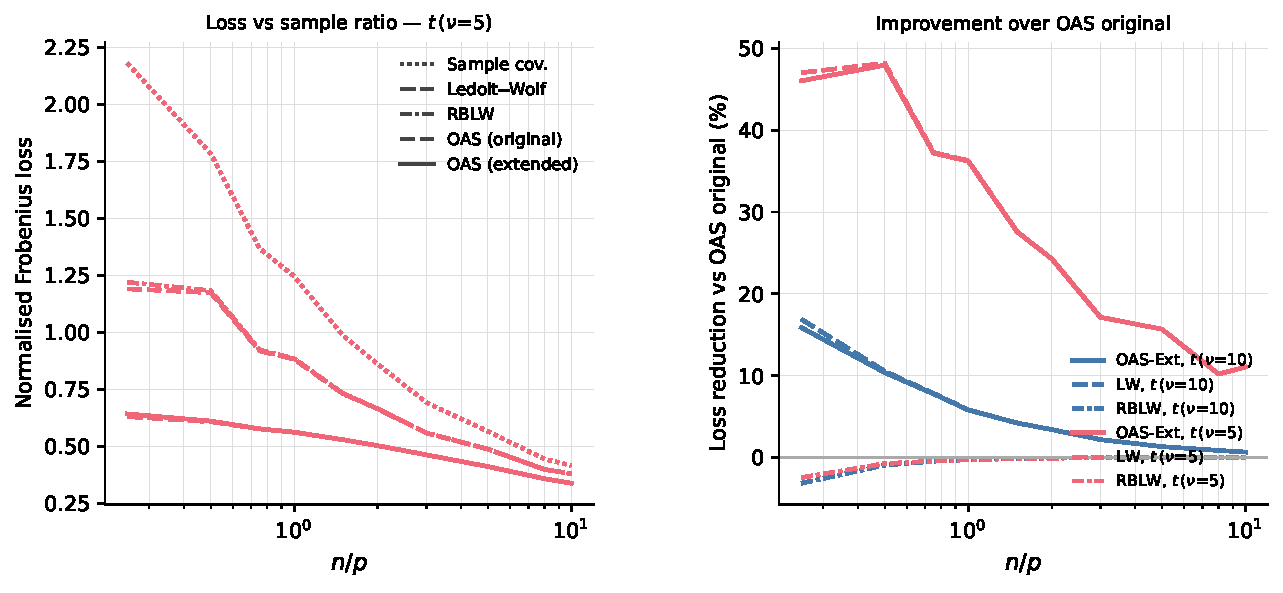
\includegraphics[width=\textwidth]{oas_simulation.pdf}
\caption{Left: normalized Frobenius loss vs.\ $n/p$ for $t(\nu\!=\!5)$ data ($p=120$),
all five estimators (dotted $=$ sample cov., long-dash $=$ LW, dash-dot $=$ RBLW,
dashed $=$ OAS, solid $=$ OAS-Extended).
Right: relative loss reduction vs.\ OAS (\%) for OAS-Extended (solid), LW (long-dash),
and RBLW (dash-dot), blue $=t(\nu\!=\!10)$, red $=t(\nu\!=\!5)$.}
\label{fig:sim}
\end{figure*}

\section{Empirical Study: Financial Returns}\label{sec-financial}

We complement the Monte Carlo evidence with an application to daily equity returns.
The universe consists of $p=50$ large-cap US equities drawn from the S\&P~500 index,
using adjusted daily log-returns from January 2010 to December 2023 ($T=3{,}521$ days)
downloaded via \texttt{yfinance}, demeaned within each estimation window.

We adopt a rolling-window protocol with $T_{\mathrm{in}}=252$ days in-sample
(approximately one trading year, giving $n/p\approx5$) and a 21-day out-of-sample
horizon stepped monthly, yielding $N=155$ evaluation windows.
At each step we estimate the covariance matrix with each estimator and form the global
minimum variance (GMV) portfolio $\hat{w}\propto\hat{\Sigma}^{-1}\mathbf{1}$.
Performance is measured by mean annualized realized volatility.

$\hat{\alpha}$ is positive in every window (median $9.0\times10^{-5}$,
mean $6.5\times10^{-4}$), confirming the heavy-tailed character of equity returns.
The largest values coincide with periods of elevated market stress; the spike in early 2020
corresponds to the COVID-19 market dislocation.

Table~\ref{tab:financial} reports realized volatility.
OAS-Extended reduces volatility by 2.0\% relative to OAS (13.28\% vs.\ 13.55\%),
approaching LW (13.276\%), with improvement highly significant ($t=3.83$, $p<0.001$;
bootstrap 95\% CI for the mean variance reduction: $[2.0,5.0]\times10^{-6}$).
RBLW closely tracks OAS ($t=3.88$, $p<0.001$), but its mean variance reduction is
more than 30 times smaller than OAS-Extended's and the bootstrap CI rounds to zero
at six decimal places --- statistically detectable but economically negligible,
confirming that neither RBLW nor OAS provides a meaningful non-Gaussian correction.

Table~\ref{tab:regime} breaks results down by market regime (VIX threshold $=20$;
99 calm windows, 56 stress windows).
In calm windows the correction yields a 1.0\% vol reduction.
In stress windows this rises to 4.0\%, approximately four times larger.
This concentration of the gain in high-$\hat{\alpha}$ periods is the direct empirical
counterpart of the theory: when heavy-tailed behavior is most pronounced, the correction
to the shrinkage intensity matters most.

\begin{table}[ht]
\centering
\caption{Mean annualized realized GMV volatility (\%), $p=50$, $N=155$ windows.
Lower is better.}
\label{tab:financial}
\begin{tabular}{lccccc}
\toprule
& S & LW & RBLW & OAS & OAS-E \\
\midrule
All ($N=155$) & 13.972 & 13.276 & 13.551 & 13.552 & 13.282 \\
\bottomrule
\end{tabular}
\end{table}

\begin{table*}[ht]
\centering
\caption{Mean annualized realized GMV volatility (\%) and percentage vol reduction
relative to OAS, by market regime (VIX threshold $=20$).}
\label{tab:regime}
\begin{tabular}{lcccccc}
\toprule
Regime & $N$ & OAS & LW & \multicolumn{1}{c}{RBLW} & OAS-E \\
\midrule
Calm (VIX $< 20$)      & 99 & 13.785 & 13.645 ($+1.0\%$) & 13.784 ($+0.0\%$) & 13.649 ($+1.0\%$) \\
Stress (VIX $\geq 20$) & 56 & 13.131 & 12.596 ($+4.1\%$) & 13.129 ($+0.0\%$) & 12.607 ($+4.0\%$) \\
\bottomrule
\end{tabular}
\end{table*}

\begin{figure*}[ht]
\centering
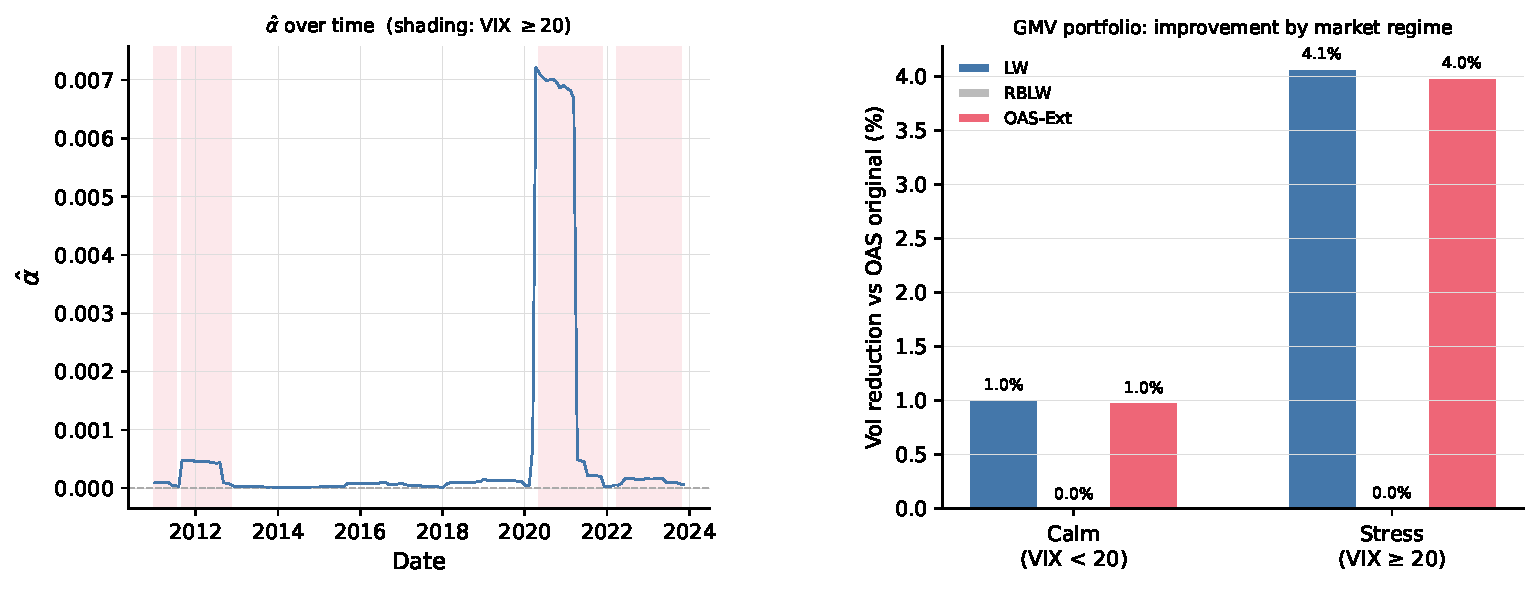
\includegraphics[width=\textwidth]{oas_financial.pdf}
\caption{Left: rolling-window $\hat{\alpha}$ for $p=50$ large-cap US equities
(January 2010 -- December 2023), stress periods (VIX $\geq20$) shaded red.
Right: percentage improvement in GMV realized volatility over OAS by market regime.
OAS-Extended and LW deliver $\sim$1\% in calm and $\sim$4\% in stress periods;
RBLW's improvement is economically negligible ($<$0.001\% in both regimes).}
\label{fig:financial}
\end{figure*}

\section{Conclusion}\label{sec-conclusion}

We have derived a closed-form correction to the Oracle Approximating Shrinkage estimator
valid for any distribution with finite fourth moments.
The correction enters through a single scalar $\alpha$ aggregating the fourth-order joint
cumulants of the data; it vanishes under Gaussianity, recovering the OAS formula
as a special case.
A consistent $O(np)$ sample estimator $\hat{\alpha}$ is available in closed form, and the
corrected shrinkage intensity lies in $[0,1]$ exactly for both the population cumulant and
its sample analogue.

Simulations and a rolling-window equity study confirm that the correction closes the gap
between OAS and Ledoit--Wolf under heavy-tailed data, with gains largest at small
$n/p$ and in high-stress market regimes.
The simulation study is limited to Student-$t$ distributions and an AR(1) covariance
structure, and the financial application covers a single universe of US large-cap equities;
generalization to other settings remains to be assessed.
The framework applies equally to neural signal covariance estimation, radar, and other
high-dimensional settings where heavy-tailed observations are common.
Natural extensions include applying the framework to structured shrinkage targets such as
factor models or banded covariance matrices, and examining the behavior of $\hat{\alpha}$
when $n/p\ll1$.

\appendix
\section{Proof That $1+\beta\geq 0$}
\label{app:proof}

\begin{proof}
Both $\operatorname{Var}(\lVert X\rVert^2)$ and $\widehat{\operatorname{Var}}(\lVert X\rVert^2)$
are non-negative (the latter by Jensen's inequality on the empirical distribution).
Writing $A$ for either $\Sigma$ or $\hat{S}$ and $V$ for the corresponding variance,
since $\alpha=V-2\operatorname{Tr}(A^2)$ we have $\alpha\geq-2\operatorname{Tr}(A^2)$.
It then suffices to show $M\geq2(1-1/p)\operatorname{Tr}(A^2)$, i.e.,
$\operatorname{Tr}^2(A)\geq\operatorname{Tr}(A^2)$.
For any positive semidefinite $A$ with eigenvalues $\lambda_i\geq0$,
\[
\operatorname{Tr}^2(A)-\operatorname{Tr}(A^2) = 2\sum_{i<j}\lambda_i\lambda_j \geq 0.
\]
Hence $1+\beta\geq0$ and $\rho_{\text{OAS-E}}\in[0,1]$.
\end{proof}

\section*{AI Use Disclosure}
The author used Claude (Anthropic) to assist with prose editing,
readability improvements, simulation code, and empirical analyses.
All mathematical derivations and intellectual contributions are
solely the author's own work.

\begin{thebibliography}{9}
\bibitem{OAS}
Y. Chen, A. Wiesel, Y. C. Eldar, and A. O. Hero, ``Shrinkage algorithms for MMSE covariance estimation,''
\emph{IEEE Trans. Signal Process.}, vol.~58, no.~10, pp.~5016--5029, Oct.~2010.

\bibitem{LW2004}
O. Ledoit and M. Wolf, ``A well-conditioned estimator for large-dimensional covariance matrices,''
\emph{J. Multivariate Anal.}, vol.~88, no.~2, pp.~365--411, 2004.

\bibitem{Ollila2017}
E. Ollila, ``Optimal high-dimensional shrinkage covariance estimation for elliptical distributions,''
in \emph{Proc. EUSIPCO}, Kos, Greece, 2017, pp.~1639--1643.

\bibitem{OllilaRaninen2019}
E. Ollila and E. Raninen, ``Optimal shrinkage covariance matrix estimation under random sampling
from elliptical distributions,''
\emph{IEEE Trans. Signal Process.}, vol.~67, no.~10, pp.~2707--2719, 2019.

\bibitem{Ollila2023}
E. Ollila, ``Linear shrinkage of sample covariance matrix under elliptical distributions: a review,''
arXiv:2308.04721, 2023.
\end{thebibliography}

\end{document}
